\RequirePackage[orthodox]{nag}
\documentclass[11pt]{article}

%% Define the include path
\makeatletter
\providecommand*{\input@path}{}
\g@addto@macro\input@path{{include/}{../include/}}
\makeatother

\usepackage{../../include/akazachk}

\title{ECH4905 ChemE Optimization HW 2}
\author{Andres Espinosa}

\begin{document}
\maketitle

\section{Problem 1}
Write the following problem in standard form
\begin{align*}
  \text{maximize} & \quad 3 x_1 + 2x_2 \\
  \text{subject to} & \quad -2x_1 + x_2 \geq 1 \\
  & \quad x_1 + 3x_2 = 2
\end{align*}
\\
\textbf{Solution: }
% TODO: SOLVE PROBLEM
To solve this problem we want to turn the above problem into the canonical form
\begin{align*}
  \text{minimize} & \quad c^\top x \\
  \text{subject to} & \quad Ax \leq b \\
  & \quad x \geq 0
\end{align*}
Flipping the maximize to minimize
\begin{align*}
  \text{minimize} & \quad -3 x_1 - 2x_2 \\
  \text{subject to} & \quad -2x_1 + x_2 \geq 1 \\
  & \quad x_1 + 3x_2 = 2
\end{align*}
Expanding the equality
\begin{align*}
  \text{minimize} & \quad -3 x_1 - 2x_2 \\
  \text{subject to} & \quad -2x_1 + x_2 \geq 1 \\
  & \quad x_1 + 3x_2 \geq 2 \\
  & \quad x_1 + 3x_2 \leq 2
\end{align*}
Flipping the $\geq$ inequalities
\begin{align*}
  \text{minimize} & \quad -3 x_1 - 2x_2 \\
  \text{subject to} & \quad 2x_1 - x_2 \leq -1 \\
  & \quad -x_1 + -3x_2 \leq -2 \\
  & \quad x_1 + 3x_2 \leq 2
\end{align*}
Bounding the variables to be $\geq 0$
\begin{align*}
  \text{minimize} & \quad -3 (x_1^+ - x_1^-) - 2(x_2^+ - x_2^-) \\
  \text{subject to} & \quad 2(x_1^+ - x_1^-) - (x_2^+ - x_2^-) \leq -1 \\
  & \quad -(x_1^+ - x_1^-) + -3(x_2^+ - x_2^-) \leq -2 \\
  & \quad (x_1^+ - x_1^-) + 3(x_2^+ - x_2^-) \leq 2 \\
  & \quad x_1^+, x_1^-, x_2^+, x_2^- \geq 0
\end{align*}
% I solved it this way by accident
To solve this problem in standard form, we turn it into
\begin{align*}
  \text{minimize} & \quad c^\top x \\
  \text{subject to} & \quad Ax = b \\
  & \quad x \geq 0
\end{align*}
We can alter the canonical form easily by adding slack variables
\begin{align*}
  \text{minimize} & \quad -3 (x_1^+ - x_1^-) - 2(x_2^+ - x_2^-) \\
  \text{subject to} & \quad 2(x_1^+ - x_1^-) - (x_2^+ - x_2^-) + s_1 = -1 \\
  & \quad (x_1^+ - x_1^-) + 3(x_2^+ - x_2^-) = 2 \\
  & \quad x_1^+, x_1^-, x_2^+, x_2^-, s_1 \geq 0
\end{align*}

\section{Problem 2}
An engineering factory makes seven products on the following machines: four
grinders, two vertical drills, three horizontal drills, one borer and one planer. Each product
yields a certain contribution to profit (defined in dollars per unit). These quantities together
with the unit production times required on each process are given below.

\begin{table}[h!]
\centering
\begin{tabular}{|c|c|c|c|c|c|c|c|}
\hline
 & P1 & P2 & P3 & P4 & P5 & P6 & P7 \\
\hline
Contribution to profit & 10 & 6 & 8 & 4 & 11 & 9 & 3 \\
\hline
Grinding (hours) & 0.5 & 0.7 & - & - & 0.3 & 0.2 & 0.5 \\
\hline
Vertical drilling (hours) & 0.1 & 0.2 & - & 0.3 & - & 0.6 & - \\
\hline
Horizontal drilling (hours) & 0.2 & - & 0.8 & - & - & - & 0.6 \\
\hline
Boring (hours) & 0.05 & 0.03 & - & 0.07 & 0.1 & - & 0.08 \\
\hline
Planning (hours) & - & - & 0.01 & - & 0.05 & - & 0.05 \\
\hline
Demand (units) & 500 & 1000 & 300 & 300 & 800 & 200 & 100 \\
\hline
\end{tabular}
\caption{Production data for the engineering factory}
\label{tab_problem2}
\end{table}

There are some marketing limitations to the production (demand), these are given as the bottom row in table \ref{tab_problem2}.
We can assume that the factory works 24 days, and that each day each machine works for
16 hours.
Formulate an LP to find the optimal product distribution.
\\
\textbf{Solution: }
% TODO: SOLVE PROBLEM
Our objective function is pretty simple and can be expressed as $10 p_1 + 6 p_2 + 8 p_3 + 4 p_4 + 11 p_5 + 9 p_6 + 3 p_7$.
To handle the constraints, we have three types: demand, machine, and non-negativity constraints.
Since the factory works 24 days and each machine works for 16 hours, each machine is constrained to work a maximum of $24 \times 16 = 384$ hours.
The optimization problem can be expressed as

\begin{align*}
  \text{maximize} & \quad 10 p_1 + 6 p_2 + 8 p_3 + 4 p_4 + 11 p_5 + 9 p_6 + 3 p_7 \\
  \text{subject to} & \quad 0.5 p_1 + 0.7 p_2 + 0.3 p_5 + 0.2 p_6 + 0.5 p_7 \leq 384 \\
  & \quad 0.1 p_1 + 0.2 p_2 + 0.3 p_4 + 0.6 p_6 \leq 384 \\
  & \quad 0.2 p_1 + 0.8 p_3 + 0.6 p_7 \leq 384 \\
  & \quad 0.05 p_1 + 0.03 p_2 + 0.07 p_4 + 0.1 p_5 + 0.08 p_7 \leq 384 \\
  & \quad 0.01 p_3 + 0.05 p_5 + 0.05 p_7 \leq 384 \\
  & \quad p_1 \leq 500 \\
  & \quad p_2 \leq 1000 \\
  & \quad p_3 \leq 300 \\
  & \quad p_4 \leq 300 \\
  & \quad p_5 \leq 800 \\
  & \quad p_6 \leq 200 \\
  & \quad p_7 \leq 100 \\
  & \quad p_1, p_2, p_3, p_4, p_5, p_6, p_7 \geq 0
\end{align*}
This can be equivalently expressed with matrix notation as 
\begin{align*}
  \text{minimize} & \quad \textbf{c}^\top \textbf{p} \\
  \text{subject to} & \quad \textbf{A} \textbf{p} \preceq 384 \times \textbf{1} \\
  & \quad \textbf{p} \preceq \textbf{d} \\
  & \quad \textbf{p} \succeq 0
\end{align*}
With the following parameters
\begin{align*}
  \textbf{c} = 
    \begin{bmatrix}
       10 \\ 6 \\ 8 \\ 4 \\ 11 \\ 9 \\ 3
    \end{bmatrix}
  \textbf{A} = 
    \begin{bmatrix}
       0.5 & 0.7 & 0 & 0 & 0.3 & 0.2 & 0.5 \\
       0.1 & 0.2 & 0 & 0.3 & 0 & 0.6 & 0 \\
       0.2 & 0 & 0.8 & 0 & 0 & 0 & 0.6 \\
       0.05 & 0.03 & 0 & 0.07 & 0.1 & 0 & 0.08 \\
       0 & 0 & 0.01 & 0 & 0.05 & 0 & 0.05
    \end{bmatrix}
  \textbf{d} = 
    \begin{bmatrix}
       500 \\ 1000 \\ 300 \\ 300 \\ 800 \\ 200 \\ 100
    \end{bmatrix}
\end{align*}
and the decision variables
\begin{align*}
  \textbf{p} = 
  \begin{bmatrix}
     p_1 \\ p_2 \\ p_3 \\ p_4 \\ p_5 \\ p_6 \\ p_7
  \end{bmatrix}
\end{align*}

\section{Problem 3}
Solve problem 2 but consider that the demand of each product is a function of
the month, i.e., that the demand for product $i$ in month $m$ is given by parameter $d_{i,m}$. In this
case, assume that you can store a maximum amount of 100 units of product each month at
a cost of 0.5/unit-month. At the beginning of the planning period there is no inventory, but at
the end we want to have 50 units of each product in storage.

When and what should the factory produce to maximize profit?
\\
\textbf{Solution: }
% TODO: SOLVE PROBLEM

\section{Problem 4}
Formulate a LP model for the following reaction network (image \ref{fig:problem_4_rn}), assuming that you want
to maximize the production rate of 3-methyltetrahydrofuran, and that you have an incoming
flux of itaconic acid equal to 1. For the sake of simplicity you can ignore the water and
hydrogen that would be required to balance the equations.
\begin{figure}[htbp]
  \centerline{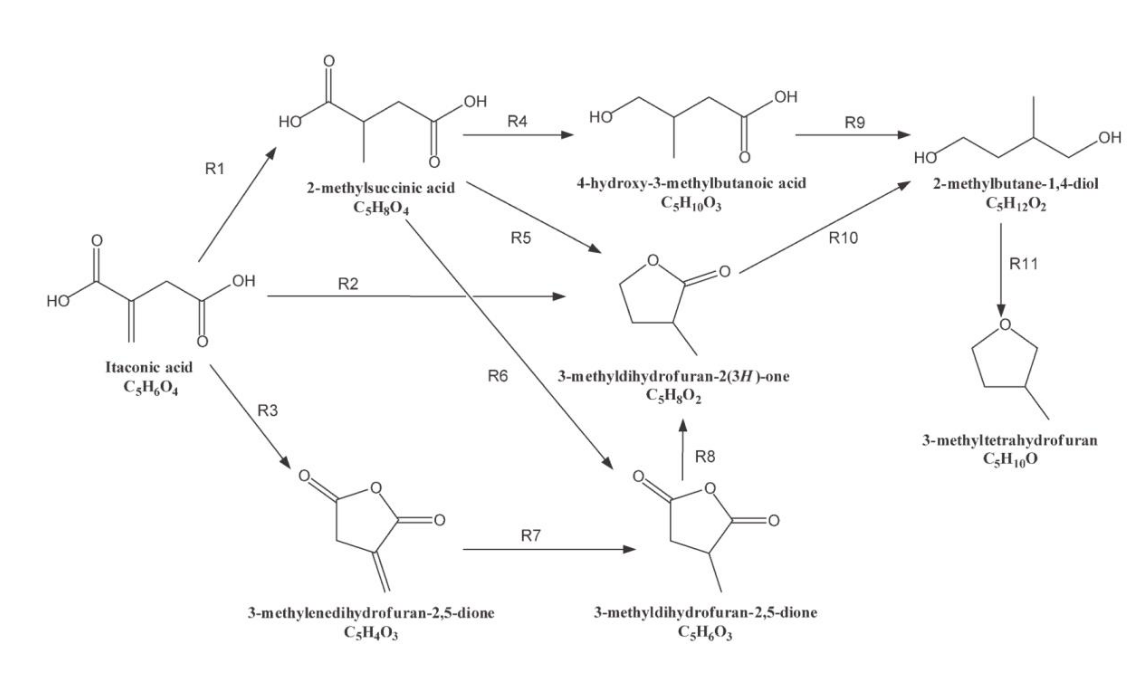
\includegraphics[width=0.75\textwidth]{images/image.png}}
  \caption{Problem 4 Reaction Network}
  \label{fig:problem_4_rn}
\end{figure}

\textbf{Solution: }
% TODO: SOLVE PROBLEM
This is a flow problem and can be modeled using the flow variables $r_i$.
\begin{align*}
  \text{maximize} & \quad r_{11} \\
  \text{subject to} & \quad 1 = r_1 + r_2 + r_3 \\
  & \quad r_1 = r_4 + r_5 + r_6 \\
  & \quad r_3 = r_7 \\
  & \quad r_6 + r_7 = r_8 \\
  & \quad r_2 + r_5 + r_8 = r_{10} \\
  & \quad r_4 = r_9 \\
  & \quad r_9 + r_{10} = r_{11}
\end{align*}


\end{document}